\documentclass[aspectratio=169,unicode]{beamer}
\usetheme{Moscow}

\usepackage[utf8]{inputenc}
\usepackage[T2A]{fontenc}
\usepackage[main=russian,english]{babel}

\usepackage{amsmath,amssymb}

\renewcommand{\thefootnote}{\fnsymbol{footnote}}
\hypersetup{
	pdfauthor={Ivan Tsybulin}
}

\usepackage{euler}
\usepackage{multirow}
\usepackage{colortbl}

\graphicspath{{images//}}

\title[Интегрирование]{Численное интегрирование}
\author[Цыбулин Иван]{Скалько Юрий Иванович\\
\textbf{Цыбулин Иван}}
\date{}

\newcommand{\colorhref}[2]{\href{#1}{\textcolor{miptbase!30!black}{#2}}}

\begin{document}

\begin{frame}[plain]
\titlepage
\end{frame}

\section{Интегрирование}
\subsection{Задача численного интегрирования}
\begin{frame}
\frametitle{Задача численного интегрирования}
	\begin{block}{Задача}
		Задана функция $f(x)$. Вычислить $\displaystyle\int_a^b f(x) dx$.
	\end{block}
	\pause

	Вначале рассмотрим случай собственного интеграла, то есть
	\begin{itemize}
		\item $a$ и $b$ --- действительные числа (не $\pm \infty$)
		\item $f(x)$ не имеет на $[a,b]$ особых точек
	\end{itemize}
	\pause

	Интеграл можно определить как предел интегральных сумм
	\[
	\int_a^b f(x) dx = \lim_{\max \Delta x_i \rightarrow 0} \sum_{i=0}^{n-1}
f(\xi_i) \Delta x_i,\quad \xi_i \in [x_i,x_{i+1}]
	\]

	\begin{center}
	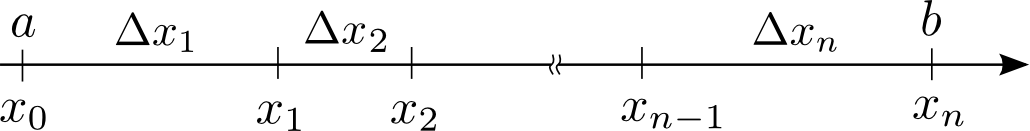
\includegraphics[height=.15\textheight]{grid.png}
	\end{center}
\end{frame}

\subsection{Численные методы}
\begin{frame}
\frametitle{Простейший численный метод}
	\[
	\int_a^b f(x) dx = \lim_{\max \Delta x_i \rightarrow 0} \sum_{i=0}^{n-1} f(\xi_i) \Delta x_i,\quad \xi_i \in [x_i,x_{i+1}]
	\]

	Введем на отрезке некоторую сетку $\left\{x_i\right\}_{i = 1}^n$. В качестве $\xi_i$ возьмем, например, середину $i$-го отрезка
	$ \xi_i = \frac{x_i+x_{i+1}}{2} $
	\pause
	\[
	\int_a^b f(x) dx \approx \sum_{i=0}^{n-1} f\left(\frac{x_i+x_{i+1}}{2}\right)\Delta x_i
	\]
	\pause

	Полученный метод называется \emph{формулой прямоугольников} или
	\emph{формулой средней точки}. Формулы численного интегрирования также
	называют \emph{квадратурными формулами}.
\end{frame}

\begin{frame}
\frametitle{Формула прямоугольников}
	\begin{figure}%
	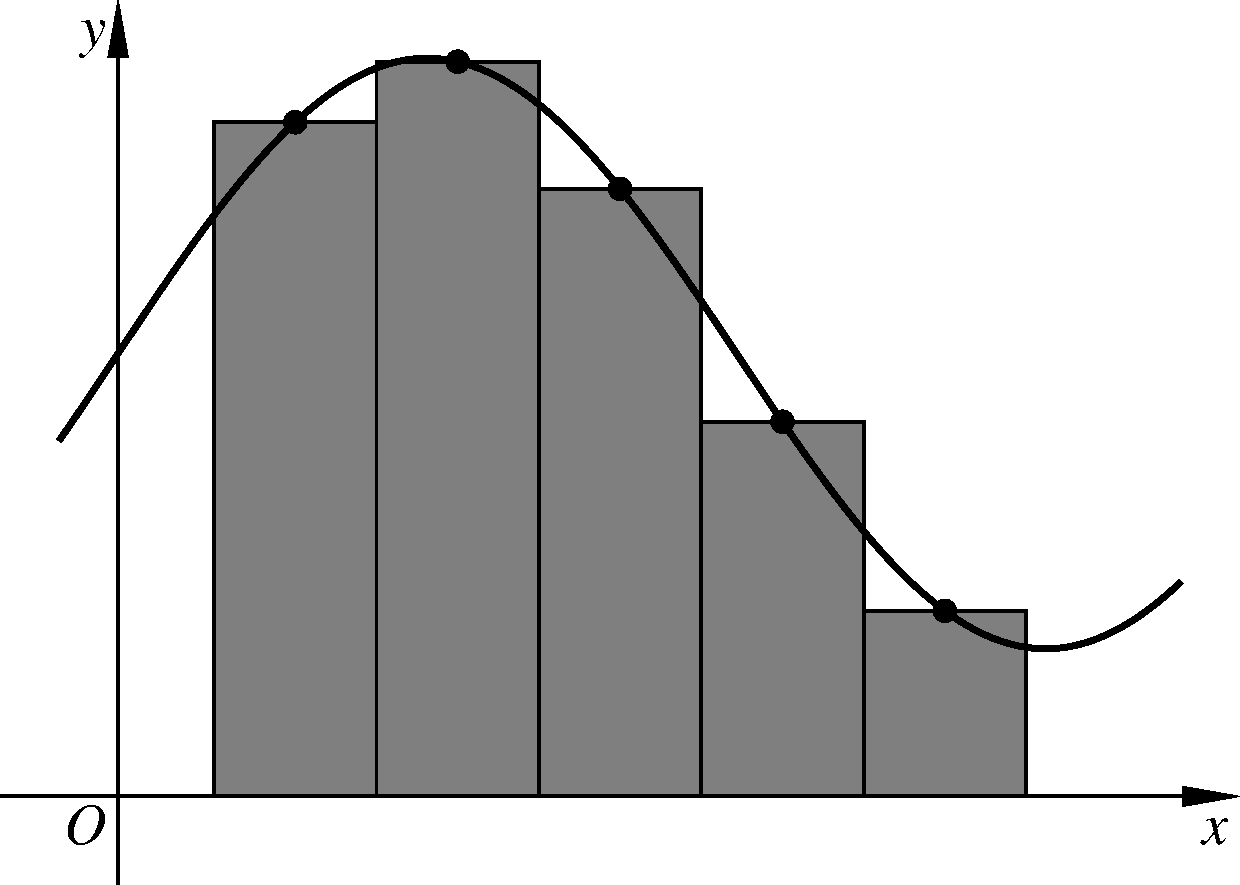
\includegraphics[height=.8\textheight]{rect.pdf}%
	\end{figure}
\end{frame}

\begin{frame}
\frametitle{Формула односторонних прямоугольников}
	Ничего не запрещает в формуле прямоугольников вместо средней точки брать крайнюю, например левую.
	Интуитивно такой выбор хуже, но к этому вернемся позднее.
	\[
	\int_a^b f(x) dx \approx \sum_{i=0}^{n-1} f\left(x_i\right)\Delta x_i
	\]
	\[
	\int_a^b f(x) dx \approx \sum_{i=0}^{n-1} f\left(x_{i+1}\right)\Delta x_i
	\]

	\pause

	Такие формулы называются формулами \emph{левых} и \emph{правых прямоугольников}
\end{frame}

\begin{frame}
\frametitle{Формулы левых и правых прямоугольников}
	\begin{figure}%
	\centering
	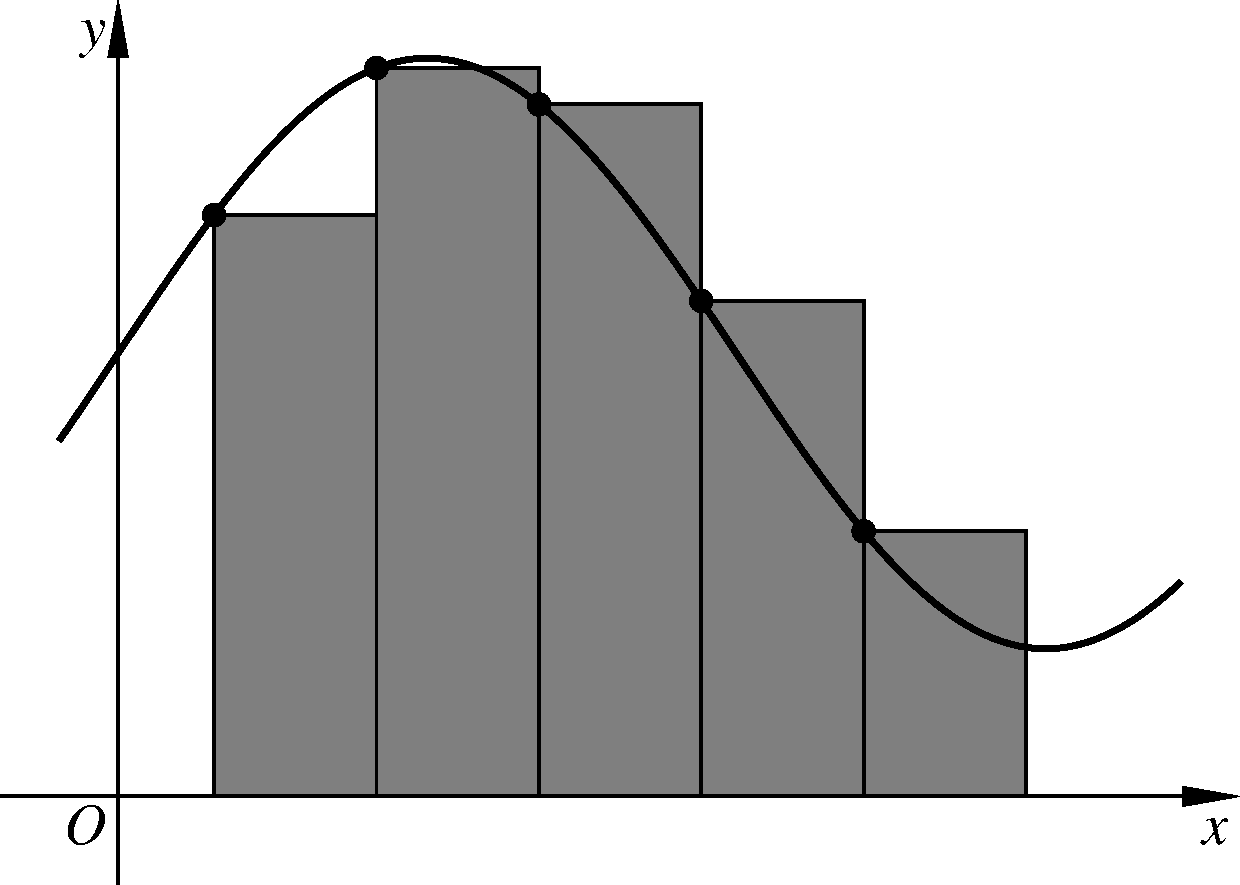
\includegraphics[width=.65\textheight]{lrect.pdf}%
	\quad
	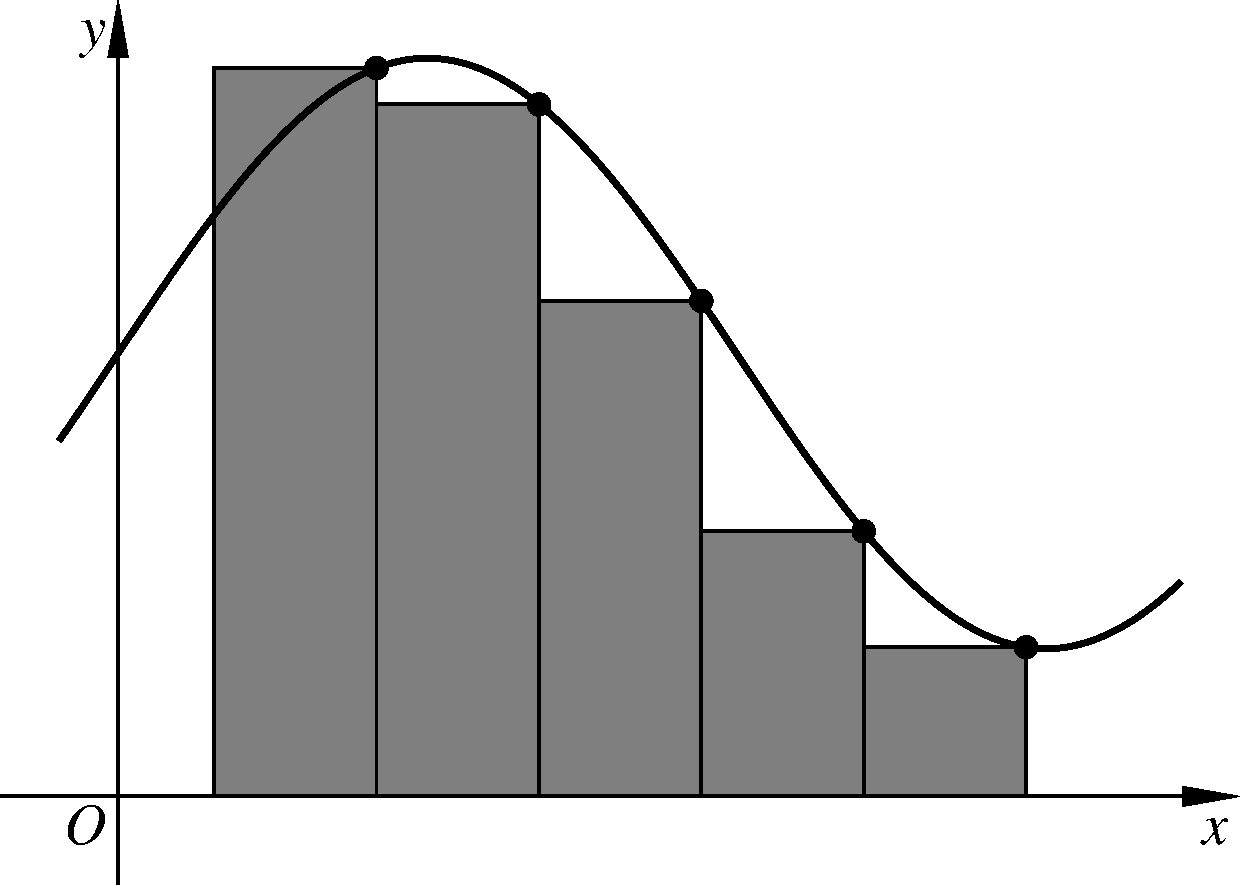
\includegraphics[width=.65\textheight]{rrect.pdf}%
	\end{figure}
\end{frame}

\subsection{Методы повышенного порядка}
\begin{frame}
\frametitle{Более точные формулы}
	Заменим функцию $f(x)$ некоторой более простой функцией $g(x)$, которая легко
	интегрируется.
	\pause

	Проще всего взять в качестве функции $g(x)$ многочлен. Тогда задача приближения
	функции $f(x)$ многочленом легко решается с помощью интерполяции.
	\pause

	Приближать функцию $f(x)$ многочленом высокой степени нежелательно,
	вследствие возможного роста ошибки интерполяции при большом числе узлов.
	Можно воспользоваться простейшим сплайном (для приближения гладкость и
	непрерывность $g(x)$ не важна) --- кусочно многочленной интерполяцией.
\end{frame}

\begin{frame}
\frametitle{Интерполяционные квадратурные формулы}
	По-аналогии с формулой прямоугольников, введем на отрезке интегрирования сетку, но теперь на каждом
	интервале приблизим функцию не константой, как в методе средней точки $f(x) \approx f\left(\frac{x_i+x_{i+1}}{2}\right)$,
	а многочленом степени $p$: $f(x) \approx Q_i(x)$.
	\[
	\int_a^b f(x) dx\approx \sum_{i=0}^{n-1} \int_{x_i}^{x_{i+1}} Q_i(x) dx
	\]
\end{frame}

\begin{frame}
\frametitle{$p=1$. Формула трапеций}
	Рассмотрим случай линейных функций $Q_i(x)$.
	\[
	Q_i(x) =
	%f(x_i)+\frac{f(x_{i+1})-f(x_i)}{x_{i+1}-x_i} (x-x_i) =
	\frac{x_{i+1}-x}{x_{i+1}-x_i} f(x_i) + \frac{x-x_i}{x_{i+1}-x_i} f(x_{i+1})
	\]
	\pause
	Проинтегрировав (представление в форме Лагранжа удобнее интегрировать), получаем
	\[
	\int_{x_i}^{x_{i+1}} Q_i(x) dx = \frac{x_{i+1}-x_i}{2} f(x_i) + \frac{x_{i+1}-x_i}{2} f(x_{i+1})
	\]
	\[
	\int_a^b f(x) dx \approx \sum_{i=0}^{n-1} \frac{f(x_i)+f(x_{i+1})}{2} \Delta x_i
	\]
	Полученная формула называется \emph{формулой трапеций}.
\end{frame}

\begin{frame}
\frametitle{Формула трапеций}
	\begin{figure}%
	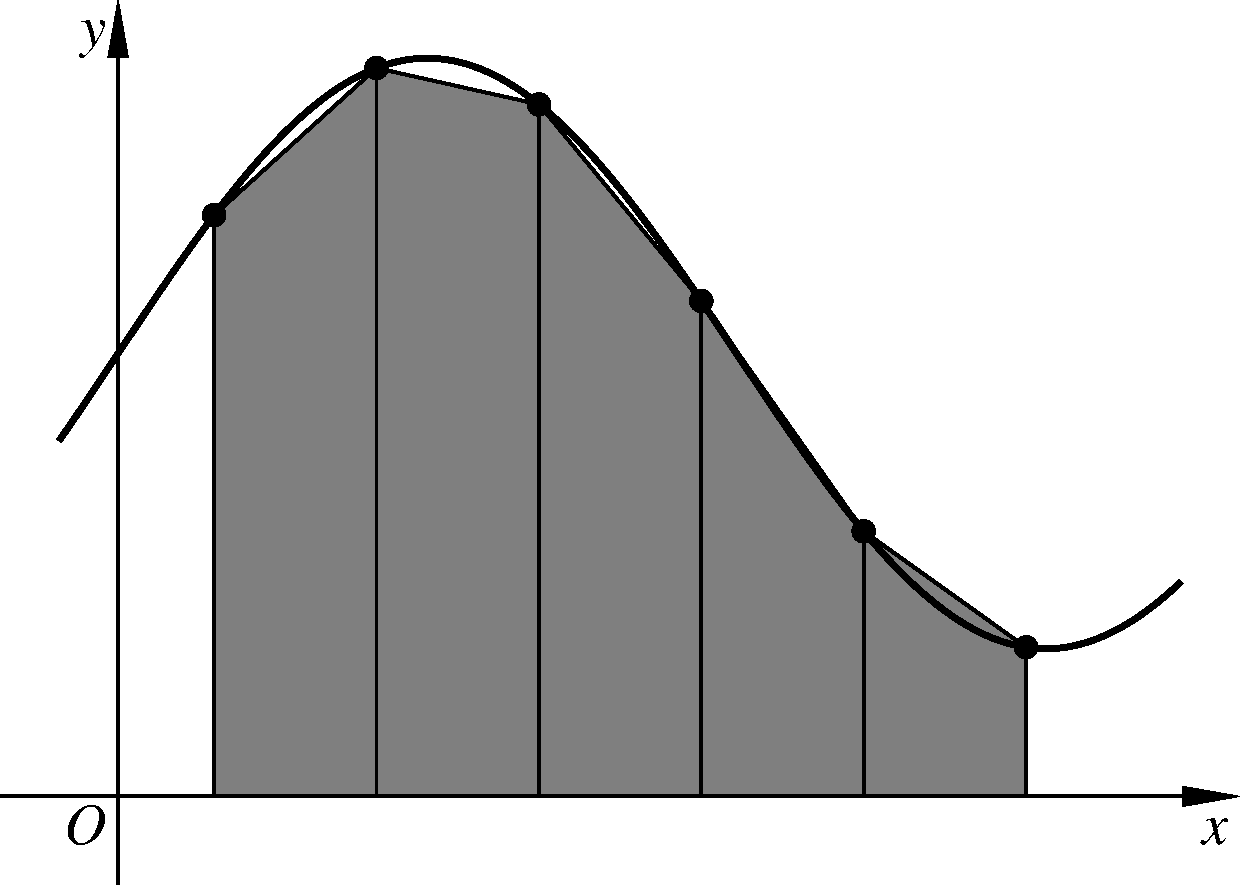
\includegraphics[height=.8\textheight]{trap.pdf}%
	\end{figure}
\end{frame}

\begin{frame}
\frametitle{Интерполяционные формулы}
	При построении формулы трапеций представление $Q_i(x)$ в виде Лагранжа оказалось
	весьма удобным. Покажем, как обобщить эту формулу на произвольный порядок $p$.
	\pause

	Введем теперь на каждом отрезке $[x_i, x_{i+1}]$ свою внутреннюю сетку из
	$p+1$ узла:
	\begin{figure}
	\centering
	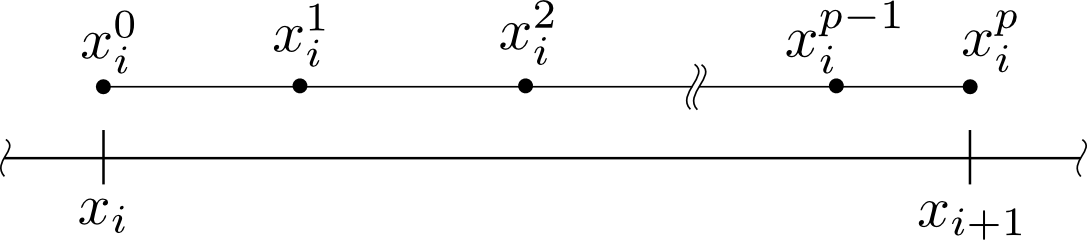
\includegraphics[width=.5\textwidth]{subgrid.png}
	\end{figure}
	\pause

	Тогда для $Q_i(x)$ справедливо представление
	\[
	Q_i(x) = \sum_{s=0}^p \ell_s(x) f(x_i^s)
	\]
	\[
	\int_{x_i}^{x_{i+1}} Q_i(x) dx = \sum_{s=0}^p f(x_i^s) \int_{x_i}^{x_{i+1}} \ell_s(x) dx
	\]
\end{frame}

\begin{frame}
\frametitle{Интерполяционные формулы}
	Интегрирование функции $Q_i(x)$ свелось к интегрированию базисных многочленов Лагранжа.
	\[
	\int_{x_i}^{x_{i+1}} Q_i(x) dx = \sum_{s=1}^p f(x_i^s) \int_{x_i}^{x_{i+1}} \ell_s(x) dx
	\]
	\pause
	Если дополнительно предположить, что на каждом отрезке внутренние сетки отличаются только масштабом
	(например, всюду равномерные или всюду чебышевские),
	то интегралы от $\ell_s(x)$ будут отличаться только множителем $\Delta x_i$
	\[
	\int_{x_i}^{x_{i+1}} \ell_s(x) dx \equiv \gamma_s \Delta x_i
	\]
	\pause
	Квадратурная формула записывается в виде
	\[
	\int_a^b f(x) dx \approx \sum_{i=0}^{n-1} \left(\sum_{s=0}^p \gamma_s f(x_i^s)\right)\Delta x_i
	\]
\end{frame}

\begin{frame}
\frametitle{$p=2$. Формула Симпсона}
	В этом случае на каждом отрезке функция приближается параболой. Для этого требуются значения в трех точках ---
	в концах отрезка и в центре. Вычисляя коэффициенты $\gamma_s$
	\[
	\gamma_0 = \frac{1}{6}, \quad \gamma_1 = \frac{2}{3}, \quad \gamma_2 = \frac{1}{6}
	\]
	и подставляя в общую формулу, получаем \emph{формулу Симпсона}
	\[
	\int_a^b f(x) dx \approx \sum_{i=0}^{n-1} \frac{f(x_i) + 4f\left(\frac{x_i+x_{i+1}}{2}\right) + f(x_{i+1})}{6} \Delta x_i
	\]
	Хотя данная формула точнее формулы трапеций и средней точки, она требует в два раза больше вычислений функции $f(x)$.
%	В случае когда сетка $\left\{x_i\right\}_{i=1}^n$ равномерная, можно пользоваться четными точками как серединами отрезков
%	вдвое большей длины $[x_{2k-1},x_{2k+1}]$.
\end{frame}

\section{Погрешность интегрирования}
\subsection{Ошибка метода}
\begin{frame}
\frametitle{Что точнее?}
	\begin{figure}%
	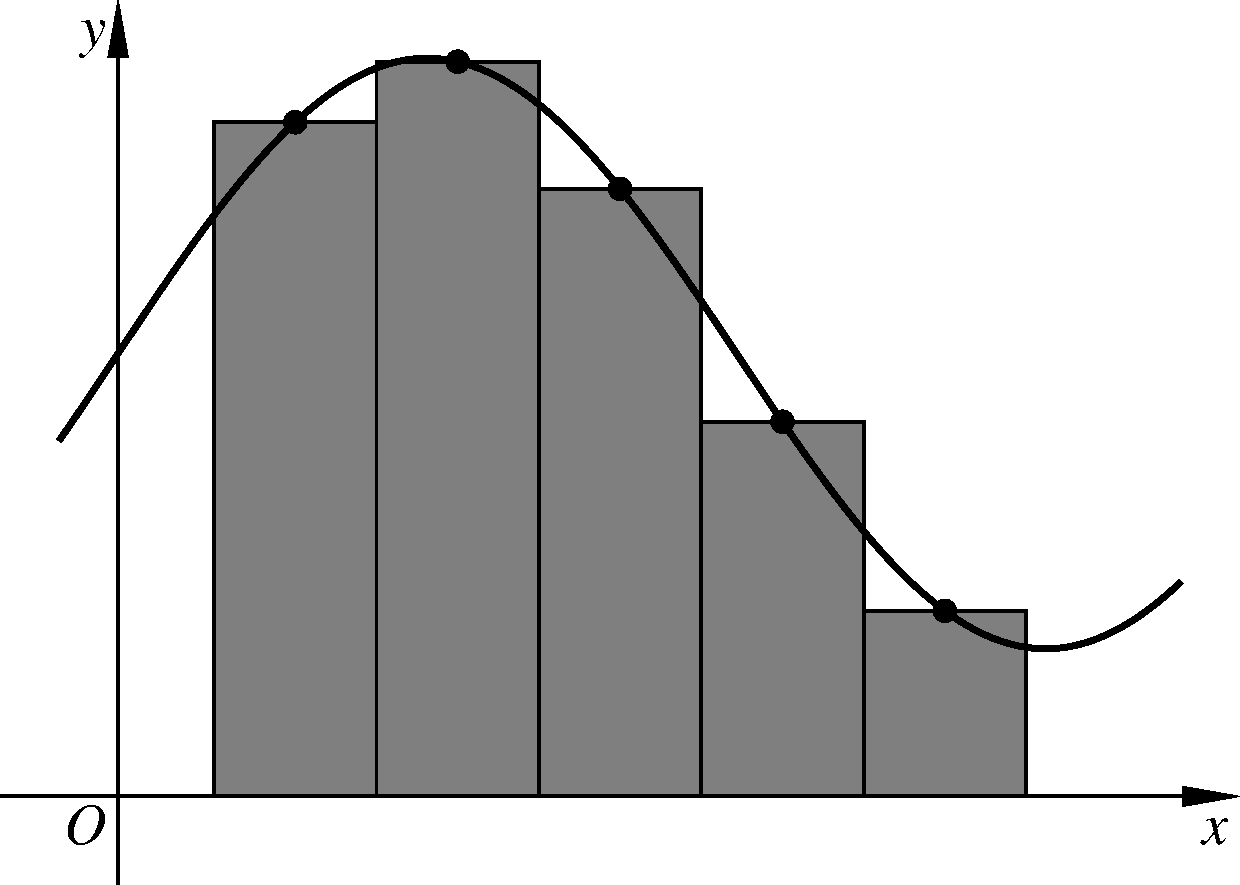
\includegraphics[width=0.5\columnwidth]{rect.pdf}%
	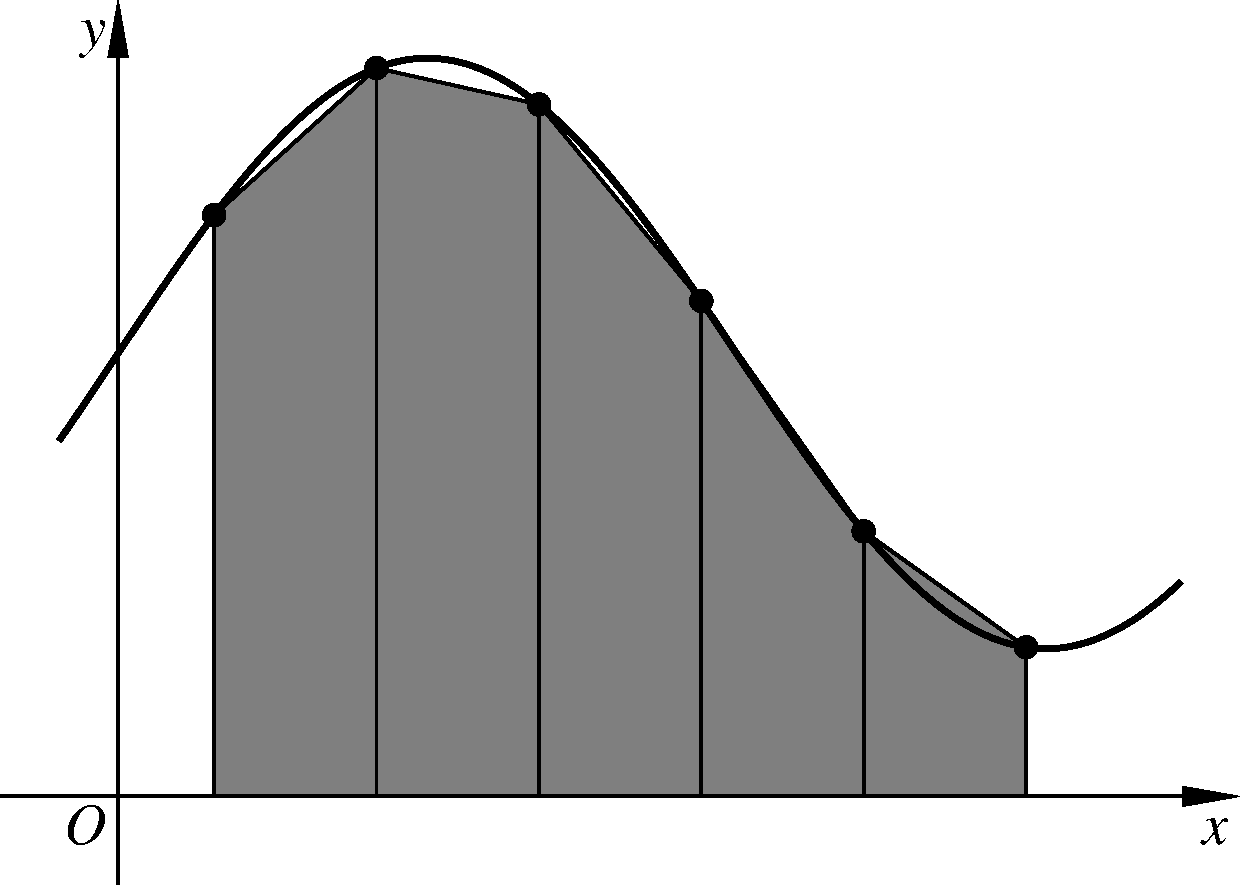
\includegraphics[width=0.5\columnwidth]{trap.pdf}%
	\end{figure}
	\pause

	\begin{columns}[c]
	\begin{column}{0.5\textwidth}
	\centering
	Ошибка $\approx 1\%$
	\end{column}
	\begin{column}{0.5\textwidth}
	\centering
	Ошибка $\approx 2\%$
	\end{column}
	\end{columns}
\end{frame}

\begin{frame}
\frametitle{Ошибка квадратурной формулы}
	Ошибка квадратурной формулы, то есть отличие точного значения интеграла от вычисленного, в худшем случае,
	просуммируется по всем интервалам сетки. Поэтому, найдем ошибку интегрирования функции только на одном отрезке.
	Для простоты, обозначим его $[a,b], \, h = b-a$.
	\[
	\int_a^b f(x) dx \approx h \sum_{s=0}^p \gamma_s f(x_s)
	\]
	\pause
	Поскольку интегрирование --- это линейная операция,
	квадратурные формулы также линейны по значениям функции $f(x)$. Здесь $\gamma_s$ --- просто некоторые
	коэффициенты квадратурной формулы.
\end{frame}

\begin{frame}
\frametitle{Ошибка квадратурной формулы}
	\[
	\int_a^b f(x) dx \approx h \sum_{s=0}^p \gamma_s f(x_s)
	\]
	Возьмем некоторую точку $z$. Конкретное значение несущественно, но удачный выбор точки $z$ может сильно сократить объем
	вычислений. \pause Представим функцию $f(x)$ в виде формулы Тейлора в окрестности точки $z$
	\[
	f(x) = f(z) + (x-z)f'(z) + \frac{(x-z)^2}{2}f''(z) + \dots + \frac{(x-z)^{m}}{m!}f^{(m)}(\zeta(x))
	\]
	Если формулу Тейлора проинтегрировать, получим
	\[
	\int_a^b f(x) dx = h f(z) + \left.\frac{(x-z)^2}{2}\right|_a^b f'(z) + \dots + \int_a^b \frac{(x-z)^{m}}{m!}f^{(m)}(\zeta(x)) dx
	\]
\end{frame}

\begin{frame}
\frametitle{Ошибка квадратурной формулы}
	\[
	\int_a^b f(x) dx = h f(z) + \left.\frac{(x-z)^2}{2}\right|_a^b f'(z) + \dots + \int_a^b \frac{(x-z)^{m}}{m!}f^{(m)}(\zeta(x)) dx
	\]
	Разложим аналогично правую часть
	\begin{align*}
		h \sum_{s=0}^p \gamma_s f(x_s) = h \sum_{s=0}^p &\gamma_s f(z) + h \sum_{s=0}^p (x_s-z)\gamma_p f'(z) + \\
	\dots&+ h \sum_{s=0}^p \gamma_s \frac{(x-z)^{m}}{m!} f^{(m)}(\zeta(x_s))
	\end{align*}
	Ошибка интегрирования получается из разности первых не совпадающих выражений перед одинаковыми производными. В частности, для всех
	квадратурных формул должно быть $\sum_{s=0}^p \gamma_s = 1$, а для формул выше первого порядка $\sum_{s=0}^p \gamma_s x_s = \frac{a+b}{2}$.
\end{frame}

\begin{frame}
\frametitle{Ошибка квадратурной формулы}
	Анализируя представления в виде формулы Тейлора, можно заключить, что
	ошибка интерполяции квадратурных формул имеет вид (для одного отрезка)
	\[
	\varepsilon_{\text{метода}} \leq C h^{r+1} M_r,
	\]
	где $C$ - некоторая числовая константа.
	Суммируя ошибку по всем отрезкам
	\[
	\varepsilon_{\text{метода}} \leq C \sum_{i=0}^{n-1} h_i^{r+1} M_{r,i} \leq C \max_i \left(M_r h^r\right)
	\sum_{i=0}^{n-1} h_i = C(b-a)\max_i \left(M_r h^r\right)
	\]
	Здесь хорошо видно, что имеет смысл уменьшать шаг $h_i$ на тех отрезках, где $r$-я производная начинает
	сильно возрастать по модулю.
\end{frame}

\subsection{Погрешность метода средней точки}
\begin{frame}
\frametitle{Погрешность метода средней точки}
	Рассмотрим один интервал $a=x_i, b=x_{i+1}$.
	Возьмем в качестве опорной именно среднюю точку $z = \frac{a+b}{2}$.
	\[
	f(x) = f(z) + (x-z)f'(z) + \frac{(x-z)^2}{2}f''(\zeta)
	\]
	\[
	\int_a^b f(x) dx = h f(z) + \int_a^b \frac{(x-z)^2}{2}f''(\zeta) dx
	\]
	\[
	\varepsilon_{\text{метод}} \leq \left|\int_a^b \frac{(x-z)^2}{2}f''(\zeta) dx \right|
	\leq M_2 \int_a^b \left|\frac{(x-z)^2}{2}\right| dx  = M_2 \frac{h^3}{24}
	\]
	При этом на всем отрезке справедлива оценка
	\[
	\varepsilon_{\text{метод}} \leq (b-a) \frac{M_2h^2}{24}
	\]
\end{frame}

\subsection{Погрешность метода трапеций}
\begin{frame}
\frametitle{Погрешность метода трапеций}
	Воспользуемся формулой Тейлора с остаточным членом в форме Пеано. В качестве опорной точки возьмем $z = \frac{a+b}{2}$
	\begin{gather*}
	f(x) = f(z) + (x-z)f'(z) + \frac{(x-z)^2}{2}f''(z) + o((x-z)^2)\\
	\int_a^b f(x) dx = h f(z) + 2\frac{(b-z)^3}{6}f''(z) + o(h^3) = hf(z) +
\frac{h^3}{24}f''(z) + o(h^3)\\
	f\left(z \pm \frac{h}{2}\right) = f(z) \pm \frac{h}{2} f'(z) + \frac{h^2}{8}
f''(z) + o(h^2)\\
	h\frac{f(a)+f(b)}{2} = hf(z) + \frac{h^3}{8} f''(z) + o(h^3)
	\end{gather*}
	Вычитая разложение квадратуры из разложения интеграла получаем ошибку
	\[
	\Delta = \frac{h^3}{24}f''(z) - \frac{h^3}{8}f''(z) + o(h^3) = -\frac{h^3}{12}f''(z) + o(h^3).
	\]
\end{frame}

\begin{frame}
\frametitle{Погрешность метода трапеций}
	Мы показали, что в пределах одного отрезка
	\[
	\int_a^b f(x) dx = h\frac{f(a)+f(b)}{2} - \frac{h^3}{12}f''\left(\frac{a+b}{2}\right) + o(h^3)
	\]
	Оценка через остаточный член в форме Лагранжа дает ошибку в два раза большую
	\[
	\varepsilon_{\text{метод}} \leq \frac{M_2 h^3}{6}
	\]
	Однако, более тонкими рассуждениями можно показать, что
	\[
	\int_a^b f(x) dx = h\frac{f(a)+f(b)}{2} - \frac{h^3}{12}f''(\xi)
	\]
	то есть асимптотическая оценка является точной.  На всем отрезке верна оценка
	\[
	\varepsilon_{\text{метод}} \leq (b-a) \frac{M_2 h^2}{12}
	\]
\end{frame}

\subsection{Погрешность метода Симпсона}
\begin{frame}
\frametitle{Погрешность метода Симпсона}
	Аналогично, для метода Симпсона без дополнительных точек можно получить
	асимптотическую оценку на интервалах
	\[
	\varepsilon_{\text{метод}} = \frac{f^{IV}(z) h^5}{180} + o(h^5)
	\]
	Эта оценка также допускает строгое обоснование
	\[
	\varepsilon_{\text{метод}} \leq \frac{M_4 h^5}{180},
	\]
	а на всем отрезке $[a,b]$
	\[
	\varepsilon_{\text{метод}} \leq (b-a)\frac{M_4 h^4}{180}
	\]
	Добавление середин отрезков эффективно уменьшает $h$ вдвое
	\[
	\varepsilon_{\text{метод}} \leq (b-a)\frac{M_4 h^4}{2880}
	\]
\end{frame}

\begin{frame}
\frametitle{Погрешность при недостаточной гладкости $f(x)$}
	Поскольку разложения в ряды Тейлора справедливы только
	при наличии у функции определенной гладкости,
	многие оценки теряют свою силу при недостаточной гладкости
	подынтегральной функции. В этом случае необходимо выводить новые оценки пользуясь
	<<урезанными>> рядами Тейлора, записанными вплоть до последней существующей производной.

	Например, метод Симпсона, примененный к функции с неограниченной 4й производной допускает оценку погрешности
	\[
	\varepsilon_{\text{метод}} \leq (b-a)\frac{M_3 h^3}{36}
	\]
	вместо
	\[
	\varepsilon_{\text{метод}} \leq (b-a)\frac{M_4 h^4}{180}
	\]
\end{frame}

\subsection{Правило Рунге}
\begin{frame}
\frametitle{Подбор шага интегрирования}
	Априорные оценки для ошибки интегрирования вида
	\[
		\varepsilon = (b-a)\frac{M_r h^r}{C}
	\]
	не всегда удобны, поскольку величины $M_r$ не всегда известны либо вычисляются
	слишком сложно. Иногда удобнее оценивать ошибку прямо в процессе вычисления интеграла.

	Пусть $I_h$ --- значение интеграла, вычисленное по некоторой квадратурной
	формуле порядка $p$, а $I^*$ --- точное значение этого интеграла. Тогда
	\[
		I_h = I^* + c h^p,
	\]
	где $c$ --- некоторый множитель, который слабо зависит от $h$. Можно считать,
	что $c$ --- константа.
\end{frame}

\begin{frame}
\frametitle{Подбор шага интегрирования}
	На сетке с шагом $h$ приближенное значение интеграла имеет погрешность $ch^p$:
	\[
		I_h = I^* + c h^p, \qquad \varepsilon_h = c h^p.
	\]
	Воспользуемся той же самой квадратурной формулой, но на вдвое более мелкой
	сетке:
	\[
		I_{h/2} = I^* + 2^{-p} c' h^p \approx I^* + 2^{-p} c h^p, \qquad
		\varepsilon_{h/2} \approx 2^{-p} \varepsilon_h
	\]
	Здесь равенство приближенное, в силу слабой зависимости $c$ от $h$.

	На практике значения $I_{h}, I_{h/2}$ известны, а $I^{*}, \varepsilon_{h},
	\varepsilon_{h/2}$ --- нет. Но разность $I_h - I_{h/2}$ в точности равна
	разности ошибок $\varepsilon_h - \varepsilon_{h/2}$:
	\[
		\Delta_{h/2} = |I_h - I_{h/2}| = |\varepsilon_{h} - \varepsilon_{h/2}| \approx
		(2^p - 1) \varepsilon_{h/2}
	\]
	Таким образом получается апостериорная оценка ошибки интегрирования
	\[
		\varepsilon_{h/2} = \frac{|I_h - I_{h/2}|}{2^p - 1}.
	\]
\end{frame}

\begin{frame}
	Мы вывели апостериорную ошибку интегрирования, в которую входит только одна
	величина --- порядок квадратурной формулы $p$.
	\[
		\varepsilon_{h/2} = \frac{|I_h - I_{h/2}|}{2^p - 1}.
	\]
	Однако, применять эту формулу нужно с осторожностью. Не всегда фактический
	порядок сходимости будет совпадать с формальным порядком метода. Полезно
	обращать внимание на величину $\varepsilon_{h} / \varepsilon_{h/2}$. Она должна
	быть близка к $2^p$, тогда можно утверждать что метод действительно сходится с
	требуемым порядком.

	В случае, когда фактический порядок сходимости меньше $p$, данная формула
	недооценивает погрешность.
\end{frame}

\begin{frame}
\frametitle{Правило Рунге}
	На основании апостериорной формулы Рунге сформулировал следующий практический
	алгоритм решения задачи интегрирования с заданной точностью $\varepsilon$:
	\begin{enumerate}
	\item Задать некоторый крупный шаг $h := h_0$ (например, $h_0 = \frac{b-a}{10}$)
	\item Вычислить интеграл с этим шагом $I_1 := I_{h}$
	\item Вычислить интеграл с половинным шагом $I_2 := I_{h / 2}$
	\item Составить разность $\Delta := |I_1 - I_2|$
	\item Если $\Delta < (2^p + 1)\varepsilon$, взять в качестве ответа
	$I_2$
	\item Иначе, положить $h := h / 2,\quad I_1 := I_2$, и повторить с шага 3. (Интеграл с новым
	шагом $h$ --- это интеграл со старым шагом $h/2$)
	\end{enumerate}
	Можно дополнительно контролировать, чтобы на каждой итерации алгоритма $\Delta$
	уменьшалась в $2^p$ раз.
\end{frame}

\section{Быстро осциллирующие функции}
\subsection{Проблемы}
\begin{frame}
\frametitle{Интегралы от быстро осциллирующих функций}
	\begin{block}{Задача}
		Вычислить
		\[
		\int_0^1 e^{-x^2} \sin 1000\pi x dx
		\]
	\end{block}
	\pause

	При использовании вышеописанных методов возникают следующие проблемы:
	\begin{itemize}
		\item Подынтегральная функция 1000 раз меняет знак на отрезке $[0,1]$. Узлов сетки необходимо не меньше
		\item r-я производная имеет максимум порядка $M_r \sim (1000\pi)^r$.
		\item Значение интеграла небольшое ($\approx 2.012\cdot10^{-4}$), а в вычислениях участвуют большие числа разного знака
	\end{itemize}

	В совокупности, из-за этих проблем расчет получается очень долгим и сильно неточным.
\end{frame}

\subsection{Специальный метод интегрирования}
\begin{frame}
\frametitle{Замена огибающей}
	Заменим подынтегральную функцию не многочленом, но функцией от которой можно аналитически посчитать
	интеграл.
	\pause

	В качестве такой функции можно взять $Q(x) \sin 1000\pi x$, где $Q(x)$ - многочлен.
	Такая функция легко интегрируется.
	\pause

	Пусть $e^{-x^2} = Q(x) + R(x)$, где $R(x)$ - небольшая функция.

	Оценим погрешность такой замены
	$$
	\int_0^1 e^{-x^2} \sin \omega x dx - \int_0^1 Q(x) \sin \omega x dx =
	\int_0^1 R(x) \sin \omega x dx
	$$
	$$
	\int_0^1 R(x) \sin \omega x dx = - \left.\frac{R(x) \cos \omega x}{\omega} \right|_0^1 +
	\int_0^1 R'(x) \frac{\cos \omega x}{\omega} dx
	$$
\end{frame}

\begin{frame}
\frametitle{Оценка ошибки}
	Возьмем в качестве $Q(x)$ интерполяционный многочлен функции $e^{-x^2}$. При этом функцией $R(x)$
	будет ошибка интерполяции, которая в точках $0$ и $1$ обратится в $0$.
	\[
	\int_0^1 R(x) \sin \omega x dx = - \left.\frac{R(x) \cos \omega x}{\omega} \right|_0^1 +
	\int_0^1 R'(x) \frac{\cos \omega x}{\omega} dx
	\]
	Так как $R(0)=R(1)=0$
	\[
	\int_0^1 R(x) \sin \omega x dx = \int_0^1 R'(x) \frac{\cos \omega x}{\omega} dx
	\]
	\[
	\varepsilon_{\text{метод}} = \left| \int_0^1 R(x) \sin \omega x dx \right| \leq \frac{1}{\omega} \max_{x\in[0,1]} |R'(x)|.
	\]
	Даже при небольшом числе узлов интерполяции ($n \sim 5 \div 10$) оценка для интеграла мала за счет множителя $\frac{1}{\omega}$.
\end{frame}

\section{Несобственные интегралы}
\subsection{Особенности}
\begin{frame}
\frametitle{Интегрирование особенностей}
	Рассмотрим теперь задачу вычисления несобственного интеграла, то есть интеграла с особенностью.
	\pause
	\begin{block}{Задача}
		Вычислить
		\[
		\int_a^b f(x) dx
		\]
		при $\lim_{x \rightarrow a}f(x) = \infty$
	\end{block}
	\pause

	Другие типы особенностей могут быть сведены к этой с использованием подходящей замены переменной.
\end{frame}

\subsection{Выделение особенности}
\begin{frame}
\frametitle{Универсальный метод выделения особенности}
	Идея метода %
	%	\footnote{он же <<Метод грамотного студента>> \textcopyright Р.П. Федоренко }
	проста --- нужно аналитически проинтегрировать особенность
	в окрестности точки $a$. Для этого в окрестности точки $a$ нужно представить
	подынтегральную функцию в виде отрезка степенного ряда.

	За пределами этой окрестности интеграл считается с применением стандартных средств для
	неособых интегралов.
\end{frame}

\begin{frame}
\frametitle{Универсальный метод выделения особенности}
	Для примера возьмем интеграл
	\[
	\int_0^1 \frac{\cos x}{\sqrt{x}} dx
	\]
	\pause

	Разобьем его на два
	\[
	\int_0^1 \frac{\cos x}{\sqrt{x}} dx = \underbrace{\int_0^\delta \frac{\cos x}{\sqrt{x}} dx}_{I_1} +
	\underbrace{\int_\delta^1 \frac{\cos x}{\sqrt{x}} dx}_{I_2}
	\]
\end{frame}

\begin{frame}
\frametitle{Аналитический учет особенности}
	\[
	I_1 = \int_0^\delta \frac{\cos x}{\sqrt{x}} dx
	\]
	\[
	\frac{\cos x}{\sqrt{x}} \approx \frac{1 - \frac{x^2}{2} + \frac{x^4}{24}}{\sqrt{x}}
	\]
	Проинтегрируем разложение подынтегральной функции
	\[
	I_1 \approx 2\sqrt{\delta} - \frac{1}{5}\delta^{5/2} +
\frac{1}{108}\delta^{9/2}
	\]
	При этом совершается ошибка порядка следующего слагаемого в ряде:
	\[
	\varepsilon_1 = \frac{1}{4680}\delta^{13/2}
	\]
\end{frame}

\begin{frame}
\frametitle{Оценка ошибки второго интеграла}
	Для вычисления второго интеграла воспользуемся формулой прямоугольников (например)
	\[
	I_2 = \int_\delta^1 \frac{\cos x}{\sqrt{x}} dx
	\]
	Оценка для ошибки интегрирования у данного метода
	\[
	\varepsilon_2 = (1-\delta)\frac{M_2 h^2}{24} \approx \frac{M_2 h^2}{24}
	\]
	Поскольку в особенности в бесконечность обращаются все производные, максимум
	второй производной на отрезке $[\delta, 1]$ будет либо близок либо точно равен
	значению производной в точке $\delta$.
	\[
	\underset{[\delta, 1]}{M_2}\left(\frac{\cos x}{\sqrt{x}}\right) \approx
	\underset{[\delta, 1]}{M_2}\left(\frac{1}{\sqrt{x}}\right)
	= \frac{3}{4}\frac{1}{\sqrt{x}^5}\Big|_{x = \delta}
	= \frac{3}{4}\delta^{-5/2}
	\]
\end{frame}

\begin{frame}
\frametitle{Определение параметра $\delta$}
	Зададимся точностью $\varepsilon_1 + \varepsilon_2 = 10^{-6}$. При этом нет смысла
	вычислять один интеграл точнее другого, $\varepsilon_1 = \varepsilon_2 = 5\cdot10^{-7}$.

	Выберем $\delta$. Это значение не должно быть большим, иначе погрешность замены
	функции отрезком ряда становится существенной. Также значение не должно быть слишком малым,
	иначе значения функции в окрестности особенности велики и могут вносить существенную погрешность в вычисления.
	Оптимальным для нашего случая будет значение $\delta = 0.3$.
\end{frame}

\begin{frame}
\frametitle{Вычисление интеграла}
	Зная $\delta = 0.3$, оценим первый интеграл $I_1$ и его погрешность $\varepsilon_1$:
	\[
	I_1 = 2\sqrt{0.3} - \frac{1}{5}0.3^{5/2} + \frac{1}{108}0.3^{9/2} \approx
1.085627188, \quad\varepsilon_1 = 8.5 \cdot 10^{-8}
	\]

	Теперь необходимо вычислить шаг сетки $h$ для формулы прямоугольников. $h =
\sqrt{\frac{24\varepsilon_2}{M_2}} \approx 9\cdot 10^{-4}$
	\[
	I_2 = 0.72342125646
	\]
	\[
	I = I_1 + I_2 = 1.8090484\underline{45}, \quad \int_0^1 \frac{\cos
x}{\sqrt{x}} dx = 1.8090484\underline{76}
	\]
	Вычисления потребовали $800$ вычислений подынтегральной функции.
\end{frame}

\subsection{Метод регуляризации}
\begin{frame}
\frametitle{Исключение особенности из функции}
	Если в предыдущем методе для избавления от особенности мы разбивали отрезок на два части, то
	в этом методе на два слагаемых разбивается сама подынтегральная функция.
	\pause
	\[
	\int_a^b f(x) dx = \int_a^b \varphi(x) dx + \int_a^b [f(x) - \varphi(x)] dx
	\]
	\pause

	Функция $\varphi(x)$ выбирается из таких условий
	\begin{itemize}
		\item $\varphi(x)$ интегрируется аналитически
		\item $f(x)-\varphi(x)$ не содержит особенности (особенность выделена в $\varphi(x)$)
		\item $f(x)-\varphi(x)$ \emph{достаточно гладкая для применения квадратурной формулы}
	\end{itemize}
\end{frame}

\begin{frame}
\frametitle{Минимальная регуляризация}
	Вернемся к примеру
	\[
	\int_0^1 \frac{\cos x}{\sqrt{x}} dx =
	\int_0^1 \varphi(x) dx +
	\int_0^1 \left[\frac{\cos x}{\sqrt{x}}-\varphi(x)\right] dx
	\]
	\pause

	Разложим подынтегральную функцию в степенной ряд
	\[
	\frac{\cos x}{\sqrt{x}} = \frac{1-\frac{x^2}{2} + \frac{x^4}{24} + \dots}{\sqrt{x}}
	\]
	\pause
	Слагаемое $\frac{1}{\sqrt{x}}$ полностью содержит в себе особенность. Без него
	у подынтегральной функции не будет особенности в точке $0$.
\end{frame}

\begin{frame}
\frametitle{Минимальная регуляризация}
	Можно положить $\varphi(x) = \frac{1}{\sqrt{x}}, g(x) = \frac{\cos x - 1}{\sqrt{x}}$
	\[
	\int_0^1 \frac{\cos x}{\sqrt{x}} dx =
	\int_0^1 \frac{1}{\sqrt{x}} dx +
	\int_0^1 \frac{\cos x-1}{\sqrt{x}} dx = 2 + \int_0^1 \frac{\cos x-1}{\sqrt{x}} dx
	\]
	\pause
	При доопределении $g(0)=0$ новая подынтегральная функция особенности не содержит.
	\pause

	Однако, если формально оценивать погрешность метода Симпсона или метода прямоугольников возникает другая трудность ---
	у функции неограниченна вторая производная
	\[g(x) \sim -\frac{x^2}{2\sqrt{x}}, g''(x) \sim -\frac{3}{8\sqrt{x}}\]
	\pause

	Можно воспользоваться формулой оценки погрешности первого порядка
	\[
	\varepsilon = (b-a)\frac{M_1 h}{4}
	\]
\end{frame}

\begin{frame}
\frametitle{Регуляризация до гладкости}
	А можно сильнее регуляризовать функцию $f(x)$, дополнительно вычтя из нее
	не дифференцируемую дважды функцию.

	Положим $\varphi(x) = \frac{1-\frac{x^2}{2}}{\sqrt{x}}, u(x) = \frac{\cos x
- 1 + \frac{x^2}{2}}{\sqrt{x}}, u(0) = 0$
	\[
	\int_0^1 \frac{\cos x}{\sqrt{x}} dx =
	\int_0^1 \frac{1-\frac{x^2}{2}}{\sqrt{x}} dx +
	\int_0^1 \frac{\cos x-1+\frac{x^2}{2}}{\sqrt{x}} dx = \frac{9}{5} + \int_0^1 u(x) dx
	\]
	\pause
	\[u(x) \sim \frac{x^4}{24\sqrt{x}}, u''(x) \sim \frac{35x\sqrt{x}}{96},
\quad M_2(u) < \infty\]
\end{frame}

\begin{frame}
\frametitle{Использование правила Рунге}
	Однако, оценивать $M_2$ сложно, и тут помогает правило Рунге(в таблице
приведены значение интеграла с учетом аналитической добавки $9/5$):
	\[
	\begin{array}{c|c|c|c|c}
	n & I_{h} & \Delta_h = |I_{2h} - I_h|
		& p = \log_2\frac{\Delta_{2h}}{\Delta_{h}}
		& \varepsilon_h = \frac{\Delta_h}{2^p - 1} \\\hline
	10 & 1.80\underline{89908657} & \star & \star & \star\\
	20 & 1.8090\underline{340645} & 4.31988 \cdot 10^{-5} & \star & \star\\
	40 & 1.80904\underline{48724} & 1.08079 \cdot 10^{-5} & 2.00 & 3.60629 \cdot 10^{-6} \\
	\textcolor{green!50!black}{80} & 1.80904\underline{75749} & 2.70251 \cdot 10^{-6} & 2.00 &
		\textcolor{green!50!black}{9.01073 \cdot 10^{-7}}\\
	160 & 1.809048\underline{2506} & 6.75662 \cdot 10^{-7} & 2.00 & 2.25236 \cdot 10^{-7}
	\end{array}
	\]
	Метод средней точки действительно сходится как метод второго порядка для
функции $u$.
	Точное значение $I^{*} = 1.80904\underline{84756}$. С необходимой точностью
$\varepsilon = 10^{-6}$ интеграл был посчитан с использованием $80$ интервалов
на отрезке $[0, 1]$.
\end{frame}

\begin{frame}[plain]
  \begin{center}
  {\Huge Спасибо за внимание!}
  \vspace{8ex}

  Цыбулин Иван

  e-mail: \colorhref{mailto:tsybulin@crec.mipt.ru}{tsybulin@crec.mipt.ru}
  \end{center}
\end{frame}

\end{document}
